\documentclass[12pt,letterpaper]{article}
\usepackage{graphicx,textcomp}
\usepackage{natbib}
\usepackage{setspace}
\usepackage{fullpage}
\usepackage{color}
\usepackage[reqno]{amsmath}
\usepackage{amsthm}
\usepackage{fancyvrb}
\usepackage{amssymb,enumerate}
\usepackage[all]{xy}
\usepackage{endnotes}
\usepackage{lscape}
\newtheorem{com}{Comment}
\usepackage{float}
\usepackage{hyperref}
\newtheorem{lem} {Lemma}
\newtheorem{prop}{Proposition}
\newtheorem{thm}{Theorem}
\newtheorem{defn}{Definition}
\newtheorem{cor}{Corollary}
\newtheorem{obs}{Observation}
\usepackage[compact]{titlesec}
\usepackage{dcolumn}
\usepackage{tikz}
\usetikzlibrary{arrows}
\usepackage{multirow}
\usepackage{subcaption}
\usepackage{xcolor}
\newcolumntype{.}{D{.}{.}{-1}}
\newcolumntype{d}[1]{D{.}{.}{#1}}
\definecolor{light-gray}{gray}{0.65}
\usepackage{url}
\usepackage{listings}
\usepackage{color}

\definecolor{codegreen}{rgb}{0,0.6,0}
\definecolor{codegray}{rgb}{0.5,0.5,0.5}
\definecolor{codepurple}{rgb}{0.58,0,0.82}
\definecolor{backcolour}{rgb}{0.95,0.95,0.92}

\lstdefinestyle{mystyle}{
	backgroundcolor=\color{backcolour},   
	commentstyle=\color{codegreen},
	keywordstyle=\color{magenta},
	numberstyle=\tiny\color{codegray},
	stringstyle=\color{codepurple},
	basicstyle=\footnotesize,
	breakatwhitespace=false,         
	breaklines=true,                 
	captionpos=b,                    
	keepspaces=true,                 
	numbers=left,                    
	numbersep=5pt,                  
	showspaces=false,                
	showstringspaces=false,
	showtabs=false,                  
	tabsize=2
}
\lstset{style=mystyle}
\newcommand{\Sref}[1]{Section~\ref{#1}}

\title{Problem Set 1 - Applied Stats/Quant Methods 1}
\date{21-09-2022}
\author{Imelda Finn (22334657}

\begin{document}
	\maketitle
	
	\section*{Solution to Problem Set 1}

 \textit{ \texttt{R} and \texttt{Latex}.}

\section*{Question 1 }

\textit{Example Prompt.}\\

\vspace{.25cm}

\noindent Maybe you need to load in my dataset first, so let's show you how to 'present' that information. You can merely 'show' us that you read in the data by 'printing' your code. \\

\lstinputlisting[language=R, firstline=41, lastline=41]{PS01_answersIF.R}  

\vspace{.25cm}

\noindent Notice, I'm reading in only one line of code from the answers in my .R file using this code: 

\begin{verbatim}
	\lstinputlisting[language=R, firstline=40, lastline=40]{PS01_answersJZ.R}}
\end{verbatim}

\noindent If you're looking at the code in the .tex file as you investigate this example, \textbf{which you should}, you'll notice that you could also copy your code results using the \texttt{verbatim} environment (\texttt{$\backslash$begin\{verbatim\}} PASTE RESULTS HERE \texttt{$\backslash$end\{verbatim\}}). The results will look something like this:


\begin{verbatim}
STATE          Y                X1             X2              X3       
AK     : 1   Min.   : 49.00   Min.   :1053   Min.   :334.0   Min.   :326.0  
AL     : 1   1st Qu.: 68.25   1st Qu.:1698   1st Qu.:374.2   1st Qu.:426.2  
AR     : 1   Median : 81.00   Median :1897   Median :395.0   Median :568.0  
AZ     : 1   Mean   : 85.04   Mean   :1912   Mean   :404.7   Mean   :561.7  
CA     : 1   3rd Qu.:102.00   3rd Qu.:2096   3rd Qu.:419.5   3rd Qu.:661.2  
CO     : 1   Max.   :142.00   Max.   :2817   Max.   :637.0   Max.   :899.0  
\end{verbatim}
\vspace{.5cm}

\noindent You can also save figures in R, and place them in your answers that you're writing in your .tex file. First, you need to make sure your path/file name is correct, then you'll save your work when your in R (see code below).

\lstinputlisting[language=R, firstline=52, lastline=55]{PS01_answersJZ.R}  
\vspace{.25cm}
\noindent With our figure saved, we just need to render it in our .tex file, which we can do using the \texttt{figure} environment:

\begin{verbatim}
	\begin{figure}[h!]\centering
		\caption{\footnotesize Example from base plot in R.}
		\label{fig:plot_1}
		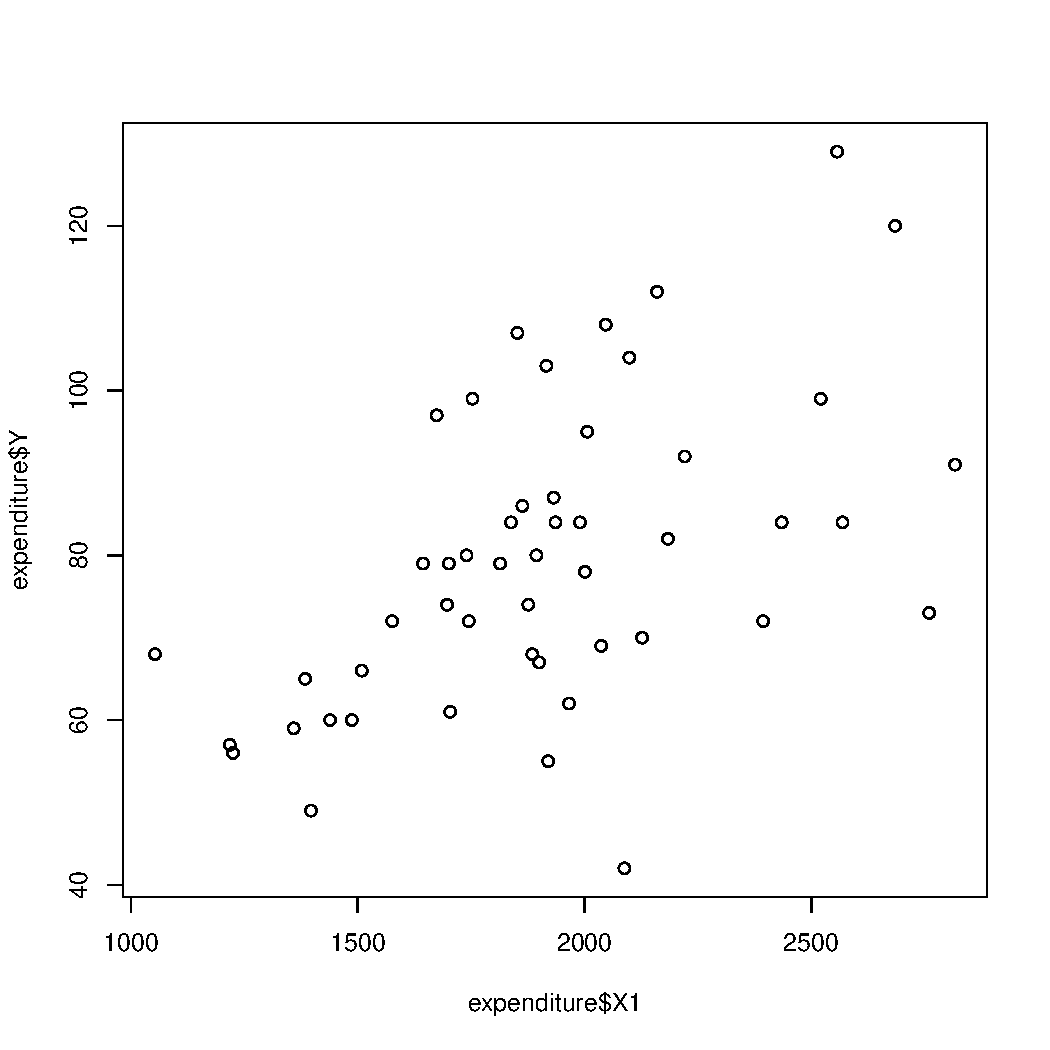
\includegraphics[width=.85\textwidth]{plot_example.pdf}
	\end{figure}
\end{verbatim}

\begin{figure}[h!]\centering
	\caption{\footnotesize Example from base plot in R.}
	\label{fig:plot_1}
	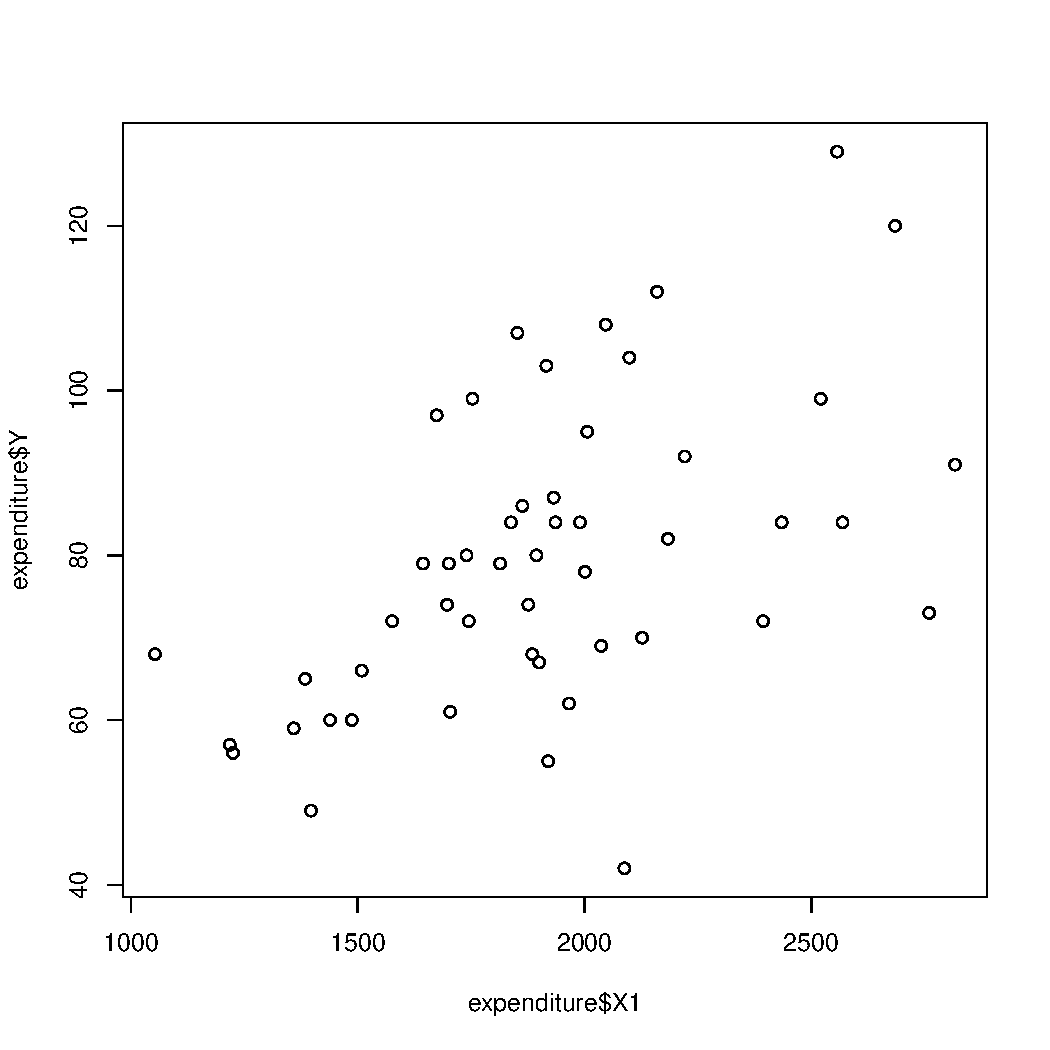
\includegraphics[width=.75\textwidth]{plot_example.pdf}
\end{figure}

\noindent Finally can also save tables in R, and place them in your answers in your .tex file, just like you would a figure. You will essentially dump and save the information in a new file, and then read that file in through Latex.

\lstinputlisting[language=R, firstline=57, lastline=66]{PS01_answersJZ.R}  

\noindent That's great, you saved your table in a new file in the same folder as your .tex and .R files. Now, let's read in our saved table using \texttt{$\backslash$input\{regression\_output1.tex\}}, which will result in:


% Table created by stargazer v.5.2.3 by Marek Hlavac, Social Policy Institute. E-mail: marek.hlavac at gmail.com
% Date and time: Thu, Sep 22, 2022 - 21:38:59
\begin{table}[!htbp] \centering 
  \caption{} 
  \label{} 
\begin{tabular}{@{\extracolsep{5pt}}lc} 
\\[-1.8ex]\hline 
\hline \\[-1.8ex] 
 & \multicolumn{1}{c}{\textit{Dependent variable:}} \\ 
\cline{2-2} 
\\[-1.8ex] & Y \\ 
\hline \\[-1.8ex] 
 X1 & 0.025$^{***}$ \\ 
  & (0.006) \\ 
  & \\ 
 Constant & 32.546$^{***}$ \\ 
  & (11.034) \\ 
  & \\ 
\hline \\[-1.8ex] 
Observations & 50 \\ 
R$^{2}$ & 0.283 \\ 
Adjusted R$^{2}$ & 0.268 \\ 
Residual Std. Error & 15.836 (df = 48) \\ 
F Statistic & 18.920$^{***}$ (df = 1; 48) \\ 
\hline 
\hline \\[-1.8ex] 
\textit{Note:}  & \multicolumn{1}{r}{$^{*}$p$<$0.1; $^{**}$p$<$0.05; $^{***}$p$<$0.01} \\ 
\end{tabular} 
\end{table}  


\noindent Or, you can paste the code you get from \texttt{stargazer} in R into the \texttt{verbatim} environment in Latex. This is more labor intensive, but produces the same results.

\end{document}
